\documentclass[11pt]{article}

\usepackage[a4paper, margin=2.3cm]{geometry}
\usepackage[T1]{fontenc}
\usepackage{lmodern}
\usepackage{microtype}
\usepackage{amsmath}
\usepackage{booktabs}
\usepackage{graphicx}
\usepackage[font=small, labelfont=bf]{caption}
\usepackage{enumitem}
\usepackage{xcolor}
\usepackage[colorlinks, linkcolor={blue!50!black}, urlcolor={blue!50!black}]{hyperref}

\graphicspath{{figures/}}
\setlength{\parindent}{0pt}
\setlength{\parskip}{5pt}
\setlist{itemsep=2pt, topsep=3pt}

\newcommand{\authorname}{Taif Ahmed Turjo}
\newcommand{\authoremail}{ahmedtaif437@gmail.com}
\newcommand{\repo}{https://github.com/taifONduty/freight-rate-forecast}
\newcommand{\code}[1]{\texttt{#1}}

\title{\textbf{Freight rate forecasting}\\[2pt]\large Spotter machine learning engineer assessment}
\author{\authorname\\\small\authoremail}
\date{October 2026}

\begin{document}
\maketitle

\section{Summary}

The task is to predict the posted rate of 12,000 truckload shipments dated November and
December 2025, using 48,000 labelled loads from January to October 2025. Every load to
predict comes after the last labelled one, so this is a two-month forecast, and I
validated it as one: five folds that each train on the past and test on the following two
months. I did not use a random split anywhere, and Section~\ref{sec:random} shows how
misleading one would have been on this data.

The final model predicts the log of the rate in three parts. A ridge regression holds
every term that has to carry past October: the daily market index and a smoothed version
of it, a linear trend, and a premium in the last month of each quarter that is larger for
flatbed and reefer loads. A gradient-boosted model then corrects the load-level pricing
from distance, weight, equipment and coordinates, and a per-lane effect, shrunk towards
zero for lanes with few loads, takes what is left. Averaged over the five folds it has a
mean absolute error of \$31.0 (1.31\%) on clean labels, against \$168 for a rate-per-mile
baseline and \$49 for gradient boosting on its own.

The data has several problems that shaped the work. The one that matters most is
\code{quote\_signal}, which is a near copy of the target in five months, its mirror image
in four, and noise in the prediction window. A random split rewards using it and a
time-based split shows that it makes forecasts worse. Beyond that, 1.4\% of the labels are
scaled by a factor of two to six, some weights have the wrong sign, a few values are
missing, and eight of the validation cities never appear in training.

\section{Data}

\subsection{The files}

\begin{table}[h]
\centering\small
\begin{tabular}{lll}
\toprule
 & Training (\code{train\_test.csv}) & To predict (\code{validation.csv}) \\
\midrule
Loads & 48,000 & 12,000 \\
Dates & 1 Jan -- 31 Oct 2025 & 1 Nov -- 31 Dec 2025 \\
Cities & 64 & 72, of which 8 unseen \\
Lanes (pickup, delivery) & 4,014 & 4,214, of which 736 unseen \\
Equipment & Dry Van 57\%, Reefer 25\%, Flatbed 18\% & same mix \\
Distance & 70 to 3,440 miles, median 953 & 70 to 3,326 miles \\
\bottomrule
\end{tabular}
\caption{The development data and the loads to predict.}
\end{table}

Each load has a pickup and delivery city with coordinates, a distance, equipment type,
weight, date, \code{market\_index} and \code{quote\_signal}. Every city has exactly one
coordinate pair. The December chart template only has city names, distance, equipment,
weight and date, so its coordinates come from a city lookup and its market index from
\code{validation.csv} (Section~\ref{sec:december}).

\subsection{Data quality}

\begin{table}[h]
\centering\small
\begin{tabular}{p{3.7cm}p{3.3cm}p{7.9cm}}
\toprule
Issue & Training / validation & Treatment \\
\midrule
Corrupted labels & 677 loads (1.4\%) / unknown & Excluded from fitting; errors reported with and without them \\
Negative weights & 292 / 145 & Sign error, absolute value taken \\
Missing weights & 300 / 165 & Median imputed inside the model, plus a missing flag \\
Missing market index & 374 / 249 & Daily mean of the index \\
\code{quote\_signal} & whole column & Dropped (Section~\ref{sec:quote}) \\
Unseen cities & -- / 12.1\% of loads & Geography through coordinates, not city names \\
\bottomrule
\end{tabular}
\caption{Data problems and how each was handled.}
\end{table}

The corrupted labels are easy to separate (Figure~\ref{fig:labels}). I fitted a plain
log-linear model of the rate on distance, equipment, weight, market index and trend, and
compared each posted rate with it. Clean loads sit between 0.87 and 1.19 times the fit.
The others sit between 2.2 and 5.4 times it (340 loads) or between 0.17 and 0.46 times it
(337 loads), with nothing in between, and they are spread evenly over months and equipment
types. I drop any load more than 1.6 times off in either direction; any cut-off inside the
gap selects the same 677 loads. The hidden November and December labels probably contain
the same corruption, which no model can predict, so I compare models on clean labels and
report the error on all labels next to it.

\begin{figure}[h]
\centering
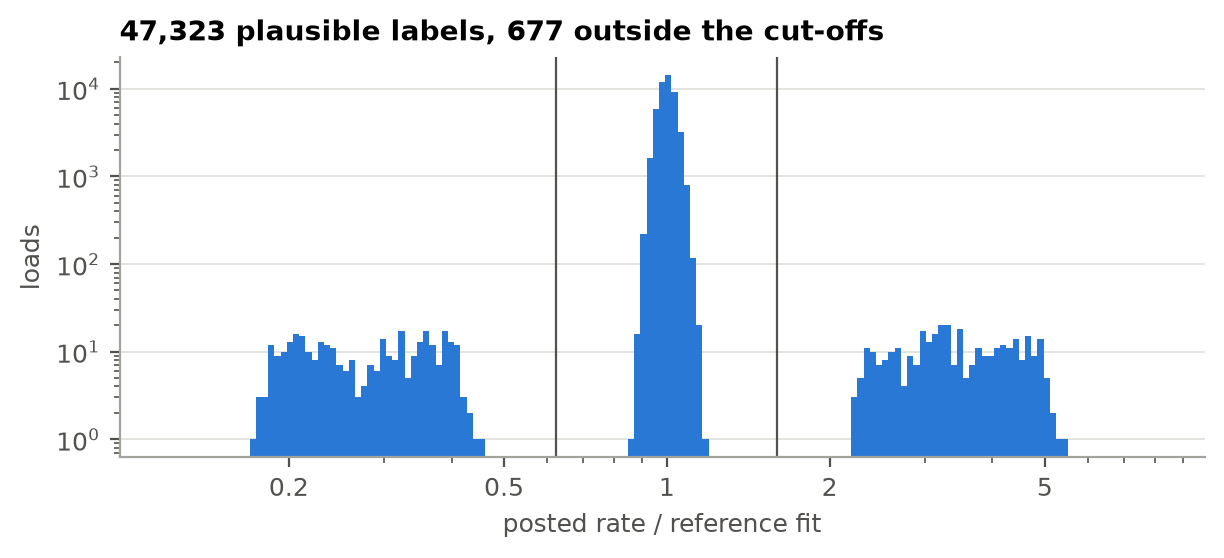
\includegraphics[width=0.9\textwidth]{label_screening.png}
\caption{Posted rate divided by a simple reference fit, both axes logarithmic. The vertical
lines are the cut-offs at 1/1.6 and 1.6.}
\label{fig:labels}
\end{figure}

Negative weights have the same magnitudes as the positive ones, and the loads price like
their heavy counterparts once the sign is flipped. Missing weights and missing index
values show no pattern by month and leave no trace in the residuals. The validation file
has roughly twice the defect rate of the training file (1.4\% missing weights against
0.6\%), so all repairs run on the prediction path as well as in training.

\code{market\_index} looks like a daily market series measured with noise on each load:
the per-load values scatter around the daily mean with a standard deviation of 0.025,
against 0.17 between days, and the scatter is unrelated to the rate. The model therefore
uses the mean over all loads on the same day, which also fills the missing values.

\subsection{The \texttt{quote\_signal} column}
\label{sec:quote}

Over the whole training set \code{quote\_signal} looks like a rate-per-mile quote with
little relation to the target (correlation 0.10). Month by month it is something else
(Figure~\ref{fig:quote}). In January, February, March, June and September it matches the
rate per mile to within about 0.02, a correlation of 0.99. In April, May, July and October
it equals 4.15 minus the rate per mile, a correlation of $-0.99$. In August it is unrelated.

What matters is which of these regimes November and December are in, and that can be
answered without labels. I correlated \code{quote\_signal} with the model's
\emph{predicted} rate per mile instead of the actual one. On the training months this
reproduces the label-based correlation almost exactly, and for November and December it
gives 0.00 and $-0.01$. The prediction window is noise, like August. A model that had
learned to use the column would apply October's mirrored relationship to noise, so I
dropped it.

\begin{figure}[h]
\centering
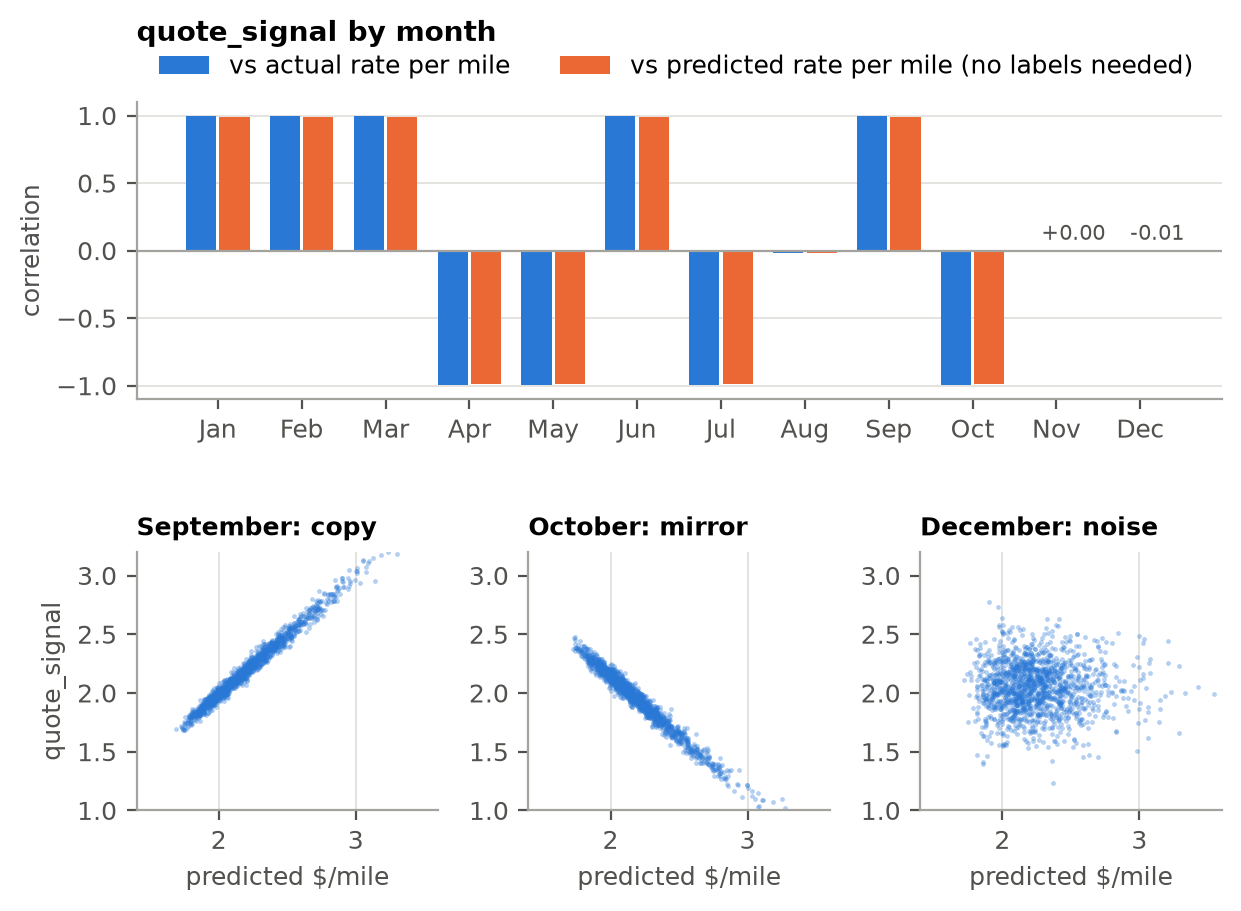
\includegraphics[width=0.9\textwidth]{quote_signal.png}
\caption{Top: monthly correlation of \code{quote\_signal} with the actual rate per mile
(training months only) and with the model's predicted rate per mile (all months). Bottom:
one month of each regime, plotted against the predicted rate per mile.}
\label{fig:quote}
\end{figure}

\subsection{What drives the rate}

\textbf{Load level.} The rate is close to a rate per mile times distance, with a discount
for distance: a dry van pays a median \$2.79 a mile on hauls of 70 to 130 miles and \$1.83
on hauls of about 2,500. Reefers cost about 12\% more than dry vans and flatbeds about
7.5\% more, and heavier loads cost slightly more. Cities carry premiums of a few percent
that follow latitude, with southern cities paying more (Figure~\ref{fig:cities}). Because
the premium changes smoothly from city to city, coordinates can price the eight cities
that only appear in validation; Section~\ref{sec:unseen} measures what that costs. Some
lanes still differ from what their two cities predict, consistently through the year;
after shrinkage these lane effects have a standard deviation of 0.55\% and reach 2.8\%.

\begin{figure}[h]
\centering
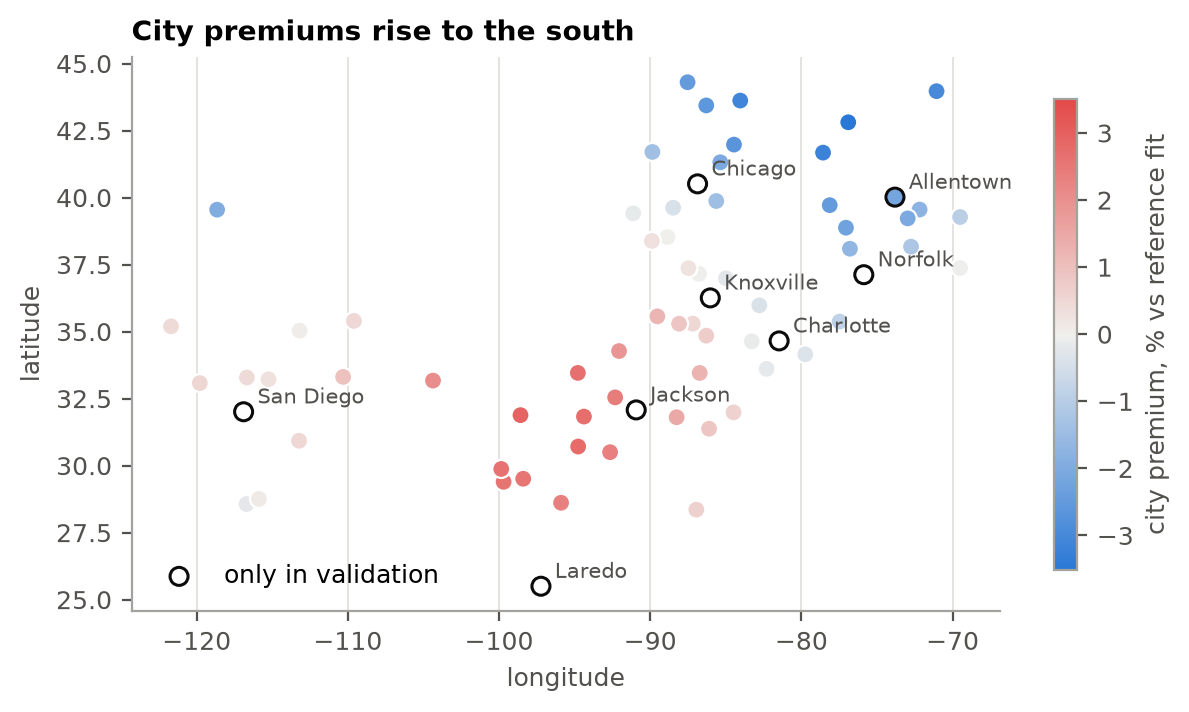
\includegraphics[width=0.9\textwidth]{city_premiums.png}
\caption{Mean residual of the reference fit for each training city, counting loads at
either end. Open circles mark the eight cities that only appear in \code{validation.csv}.}
\label{fig:cities}
\end{figure}

\textbf{Time.} Figure~\ref{fig:market} shows the daily rate level once the load-level
structure is removed, above the market index. The level follows the index, including the
fall at the end of July, and drifts upward by about 0.6\% a month on top of it. The index
has a strong weekly cycle (Sunday 0.96, Thursday 1.16 on average), and the rate does not
respond to that cycle the way it responds to the index's level. With the daily index as
its only market input, the model trained through June over-predicted August by almost 2\%
once the index had fallen (Figure~\ref{fig:tracking}). Adding an exponentially weighted
average of the log index, with a five-day half-life, lets the ridge stage price the
sustained level separately from the daily swing (Table~\ref{tab:learned}), and it cut the
error on that fold from \$40.5 to \$29.7.

\begin{figure}[h]
\centering
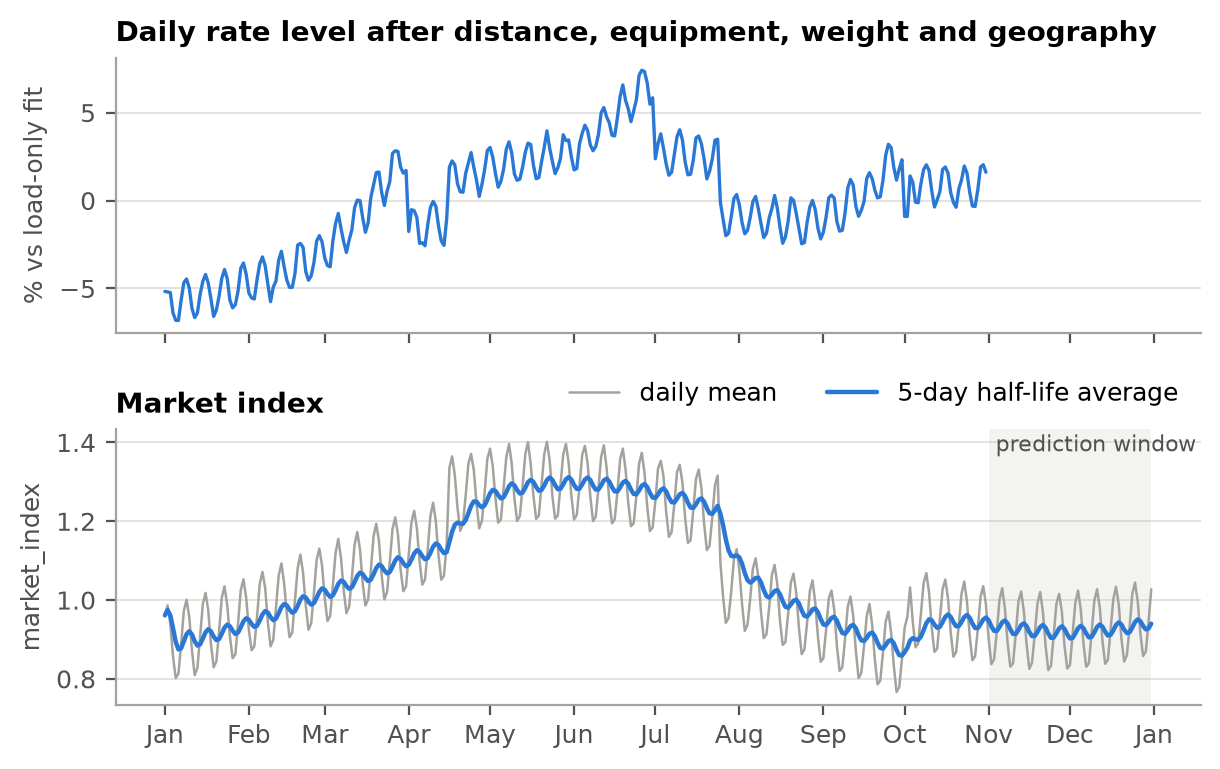
\includegraphics[width=0.9\textwidth]{market_level.png}
\caption{Top: daily mean residual of a fit on distance, equipment, weight and coordinates
only. Bottom: daily mean market index and its smoothed version; November and December are
shaded.}
\label{fig:market}
\end{figure}

The last month of every quarter is more expensive, and how much depends on the equipment
(Figure~\ref{fig:quarter}). The pattern is the same in all three complete quarters. In the
fitted model the premium on the last day of a quarter is 2.6\% for dry vans, 8.4\% for
flatbeds and 5.3\% for reefers, relative to the first two months. This matters for the
forecast because the prediction window ends on a quarter end: November is before the
premium, December is inside it, and there is no labelled December to learn from. The
model learns the premium from March, June and September and applies it to December.
Weekdays showed no effect beyond what the market index already carries, and the few
public holidays in the data showed no consistent one, so there are no holiday features.

\begin{figure}[h]
\centering
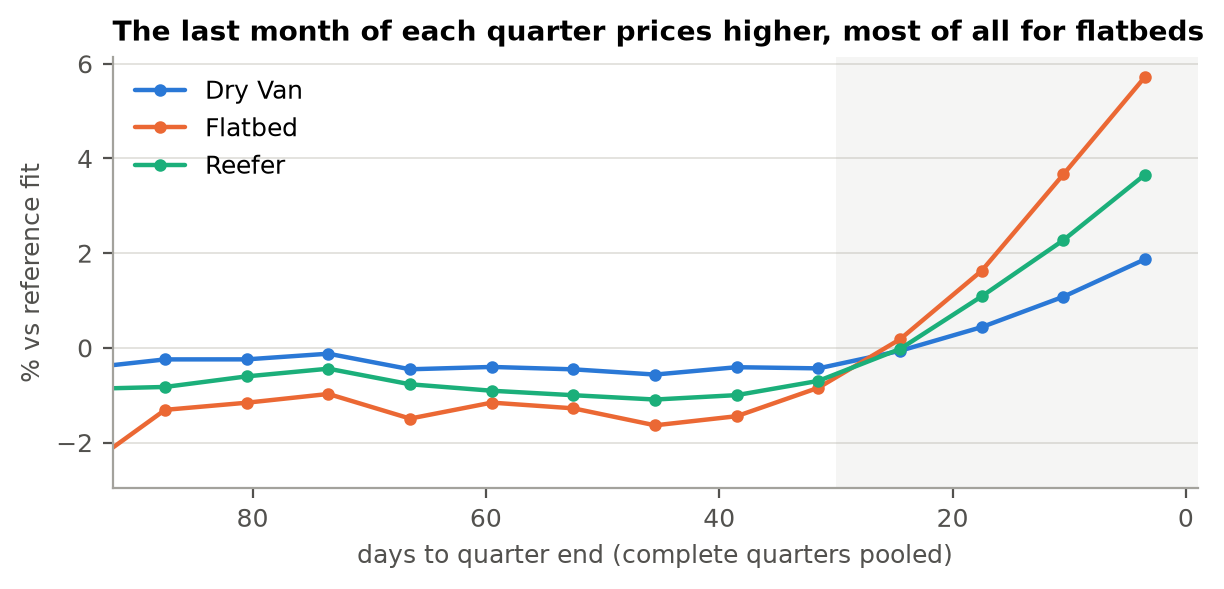
\includegraphics[width=0.9\textwidth]{quarter_end.png}
\caption{Residual of the reference fit by days to the end of the quarter, January to
September, in weekly steps. The shaded area is the last 30 days.}
\label{fig:quarter}
\end{figure}

\section{Validation design}

\subsection{Splitting the development data}

The prediction window starts the day after the training data ends and runs for two months,
so I evaluated every model the same way: train on all loads before a cut-off date and
predict the following two months. Cut-offs on the first of May, June, July, August and
September give the five folds in Table~\ref{tab:folds}. Their test months overlap, so they
are not independent, but each is a fair rehearsal of the real task and together they cover
a rising market, the July fall and a flat late summer. The May and August folds have the
same shape as the real task: training ends one month into a quarter and the test covers
the rest of it, quarter end included.

\begin{table}[h]
\centering\small
\begin{tabular}{llll}
\toprule
Fold & Trained on & Tested on & Clean test loads \\
\midrule
May--Jun & January to April & May and June & 9,571 \\
Jun--Jul & January to May & June and July & 9,567 \\
Jul--Aug & January to June & July and August & 9,538 \\
Aug--Sep & January to July & August and September & 9,297 \\
Sep--Oct & January to August & September and October & 9,379 \\
\bottomrule
\end{tabular}
\caption{Expanding-window folds, each forecasting two months ahead.}
\label{tab:folds}
\end{table}

Inside each fold the corrupted labels are screened using the training window only, so the
screening never sees the test months. I report the mean absolute error (MAE), root mean
squared error and mean absolute percentage error (MAPE) in dollars of posted rate. Model
choices were made on the clean test labels, since that is the part a model can affect;
the same metrics on all test labels are shown alongside. Once the design was fixed, I
refitted the model on all 47,323 clean training loads.

\subsection{What a random split would have said}
\label{sec:random}

To see what the split choice changes, I scored plain gradient boosting twice, with and
without the \code{quote\_signal} column, once under random five-fold cross-validation and
once under the time-based folds (Table~\ref{tab:random}).

\begin{table}[h]
\centering\small
\begin{tabular}{lrr}
\toprule
MAE on clean labels & without \code{quote\_signal} & with \code{quote\_signal} \\
\midrule
Random five-fold & \$34.3 & \$29.1 \\
Time-based folds & \$48.8 & \$53.8 \\
\bottomrule
\end{tabular}
\caption{The same model under two validation schemes.}
\label{tab:random}
\end{table}

Random cross-validation understates the forecast error of the plain model by about 30\%
(\$34.3 against \$48.8) and makes \code{quote\_signal} look like a 15\% improvement. On the
time-based folds the same column makes the error 10\% worse. A random split puts loads
from the same week on both sides, so the model can use the current regime of
\code{quote\_signal} and the current market level, neither of which is known two months
ahead.

\section{Model}

\subsection{Why this shape}

Gradient boosting is a sensible first model, but on this task its error grows the further
it forecasts (Figure~\ref{fig:bias}). A tree cannot produce a level it has never seen, so
past the last training date it keeps returning the last leaf, and in the training months
the market index and the season move together, which a tree cannot pull apart. By the end
of the forecast window it is about 1\% too low on average. A linear model extrapolates
well but describes the load-level pricing less well. The final model splits the work:
\[
\log \text{rate} = \underbrace{x_{\text{time}}^\top\beta + x_{\text{load}}^\top\gamma}_{\text{ridge}}
+ \underbrace{f(\text{load})}_{\text{gradient boosting}}
+ \underbrace{u_{\text{lane}}}_{\text{shrunk lane effect}}
\]

\begin{itemize}
\item \textbf{Ridge regression.} The log of the daily market index and its square; the
same for its exponentially weighted average (five-day half-life); a linear trend; three
hinge functions of the days to quarter end (active in the last 30, 14 and 7 days), each
also interacted with flatbed and reefer; cubic splines with linear extrapolation in log
distance and in weight; a missing-weight flag; equipment; the four coordinates.
\item \textbf{Gradient boosting} on log distance, weight, equipment and the four
coordinates, fitted to the ridge residual. It is scikit-learn's
\code{HistGradientBoostingRegressor} with 500 rounds on all the data (no early stopping),
31 leaves and a learning rate of 0.05, and it sees no date-derived feature.
\item \textbf{Lane effect.} The mean remaining residual of each pickup--delivery pair,
multiplied by $n/(n + \sigma^2/\tau^2)$, where $n$ is the lane's load count, $\sigma^2$ the
residual variance within lanes and $\tau^2$ the variance of true lane effects estimated from the spread
of lane means. Lanes never seen in training get zero.
\end{itemize}

Because the boosted stage never sees a date, any change in level after October comes from
the ridge terms and the market index, which \code{validation.csv} supplies for November
and December.

\subsection{Results}

\begin{table}[h]
\centering\footnotesize
\setlength{\tabcolsep}{4pt}
\begin{tabular}{lrrrrr|rrr|rr}
\toprule
 & \multicolumn{5}{c|}{MAE by fold} & \multicolumn{3}{c|}{Mean, clean labels} & \multicolumn{2}{c}{Mean, all labels} \\
Model & May & Jun & Jul & Aug & Sep & MAE & RMSE & MAPE & MAE & MAPE \\
\midrule
Rate per mile by equipment & 153.7 & 153.3 & 172.4 & 186.7 & 175.1 & 168.2 & 235.8 & 8.33\% & 220.7 & 10.46\% \\
Gradient boosting alone & 55.0 & 54.9 & 50.6 & 36.3 & 47.2 & 48.8 & 70.6 & 2.08\% & 102.9 & 4.35\% \\
Linear terms only & 47.4 & 46.4 & 44.1 & 43.5 & 46.4 & 45.6 & 69.0 & 1.94\% & 99.7 & 4.22\% \\
+ boosted load correction & 33.6 & 33.6 & 31.9 & 30.9 & 35.2 & 33.0 & 48.0 & 1.40\% & 87.3 & 3.68\% \\
\textbf{+ lane effects (final)} & \textbf{31.7} & \textbf{31.6} & \textbf{29.7} & \textbf{28.8} & 33.4 & \textbf{31.0} & \textbf{45.2} & \textbf{1.31\%} & \textbf{85.3} & \textbf{3.60\%} \\
\midrule
Final without smoothed index & 32.7 & 32.4 & 40.5 & 33.0 & 31.9 & 34.1 & 49.5 & 1.43\% & 88.3 & 3.73\% \\
\bottomrule
\end{tabular}
\caption{Backtest in dollars. Folds are named by their first test month. ``Linear terms
only'' is the ridge stage of the final model on its own.}
\label{tab:results}
\end{table}

Each stage improves the mean and nearly every fold (Table~\ref{tab:results}). The linear
model alone already beats gradient boosting, which says the hard part of this problem is
the time structure rather than load-level non-linearity. The smoothed index matters most
on the July--August fold, where the market falls sharply. Including the corrupted labels
raises every model's MAPE by about 2.3 points; that floor comes from the corruption, not
from the model. Across the forecast window the final model's bias stays within 0.4\%
(Figure~\ref{fig:bias}).

\begin{figure}[h]
\centering
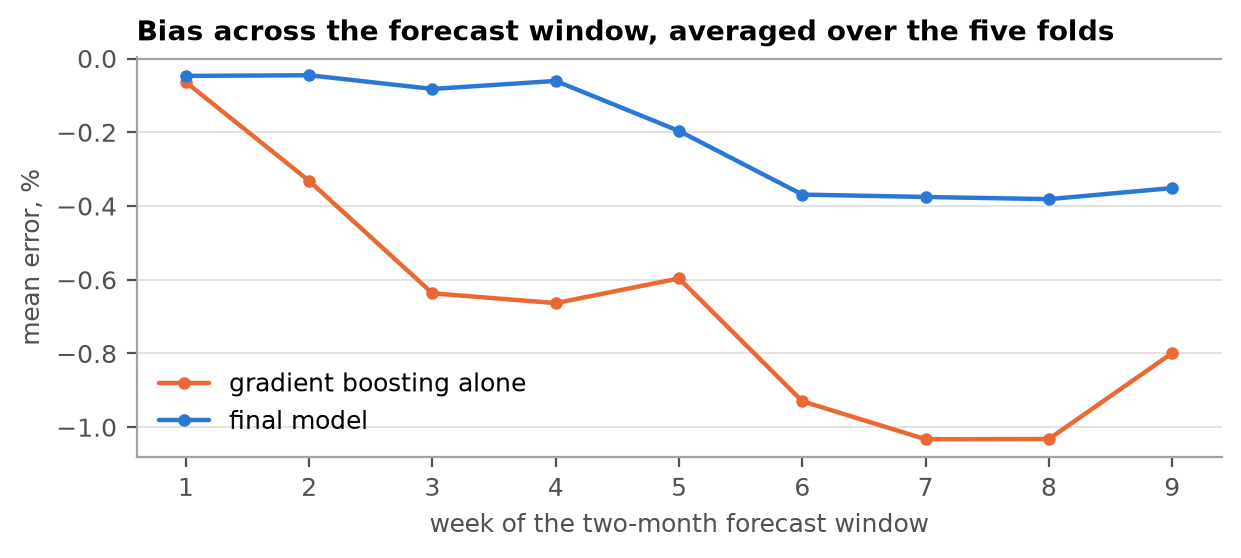
\includegraphics[width=0.9\textwidth]{horizon_bias.png}
\caption{Mean error, $100\log(\text{predicted}/\text{actual})$, by week of the forecast
window, averaged over the five folds.}
\label{fig:bias}
\end{figure}

\subsection{Forecasts against actuals}

Figure~\ref{fig:tracking} follows two folds day by day. In the July--August fold the model
without the smoothed index stays close until the market falls at the end of July and then
runs about 1.8\% too high through August; the final model follows the fall. The
September--October fold shows the final model's main weakness. It tracks September
closely, including the quarter-end rise and the drop on 1 October, neither of which is in
its training window at those dates, but it runs about 1.2\% low through October, when the
rate level rose further than the index and the trend explain.

\begin{figure}[h]
\centering
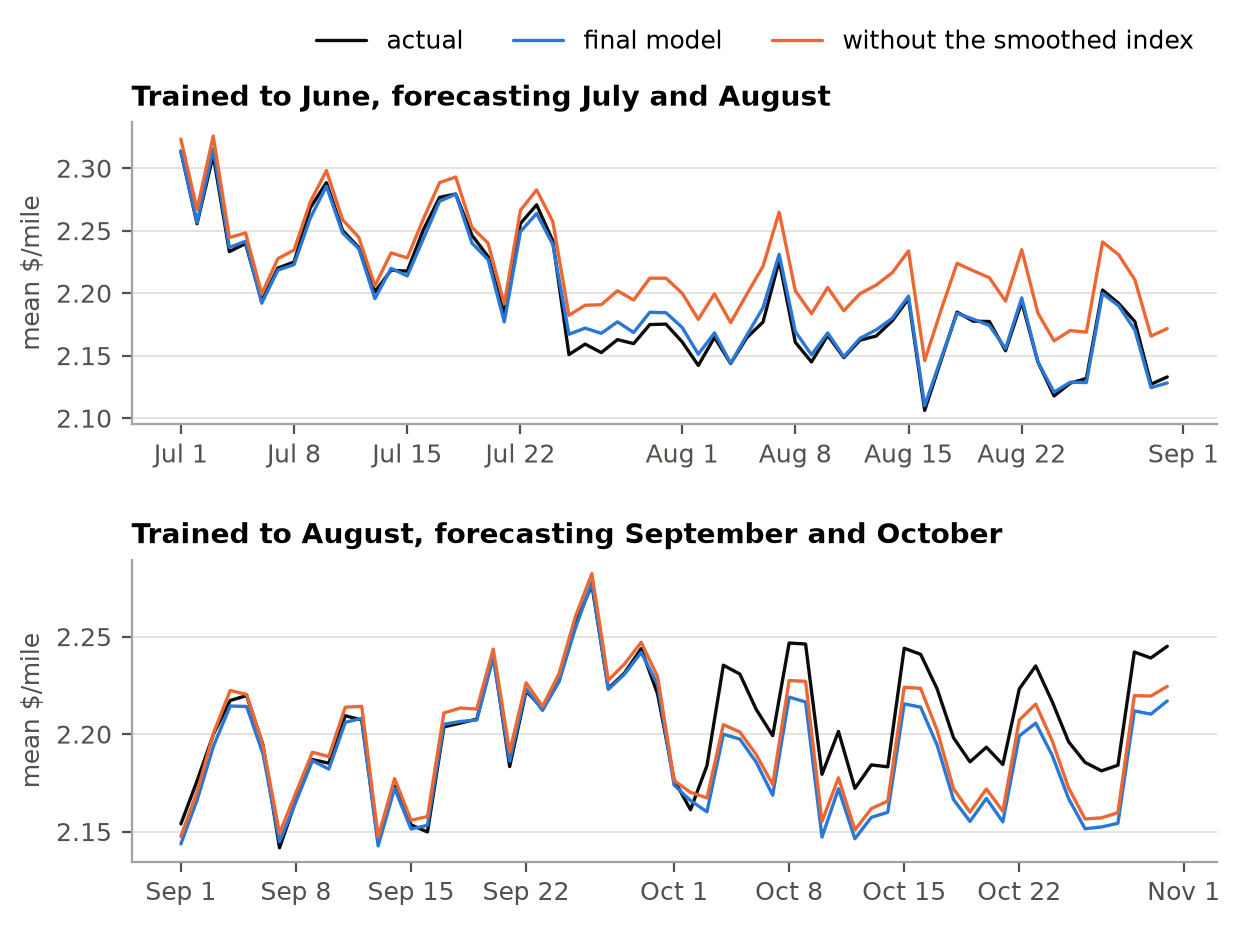
\includegraphics[width=0.9\textwidth]{forecast_tracking.png}
\caption{Daily mean rate per mile of the clean test loads against the forecasts of the
final model and of the same model without the smoothed index.}
\label{fig:tracking}
\end{figure}

\subsection{What the model learned}

The ridge stage is small enough to read (Table~\ref{tab:learned}). An elasticity of 0.13
means a 1\% rise in the market index raises the rate by 0.13\%. At ordinary index levels a
one-day move and a sustained move have about the same effect. When the market is hot the
sustained level matters much more: at an index of 1.3 a sustained move has an elasticity of
0.23, against 0.17 for a one-day swing. That difference is what the smoothed index adds. On
top of the market, the rate drifts up by 0.58\% a month. Outside the last month of a quarter
flatbeds cost 7.5\% and reefers 12.5\% more than dry vans, and the quarter-end premium in
the lower half of the table comes on top of that. The \code{train} command recomputes these
numbers and saves them in \code{report/tables}.

\begin{table}[h]
\centering\small
\begin{tabular}{lrrr}
\toprule
Elasticity to the market index & at index 0.9 & at index 1.0 & at index 1.3 \\
\midrule
One-day move & 0.12 & 0.13 & 0.17 \\
Sustained move & 0.09 & 0.13 & 0.23 \\
\midrule
Quarter-end premium & 14 days before & 7 days before & last day \\
\midrule
Dry van & 1.0\% & 1.7\% & 2.6\% \\
Flatbed & 3.7\% & 6.0\% & 8.4\% \\
Reefer & 2.3\% & 3.6\% & 5.3\% \\
\bottomrule
\end{tabular}
\caption{Market and quarter-end effects of the fitted ridge stage. A one-day move changes the
daily index only; a sustained move also carries through the smoothed index.}
\label{tab:learned}
\end{table}

\subsection{Unseen cities}
\label{sec:unseen}

Twelve percent of the validation loads touch one of eight cities the model has never seen.
To measure what that costs, I refitted the September--October fold three times, each time
without six randomly drawn training cities, and compared the test loads that touch them with
the rest (Table~\ref{tab:unseen}). Across the three draws, a load touching an unseen city is
off by 0.14 to 0.19 percentage points more, which is the price of pricing a city from its
coordinates alone. Seven of the eight real unseen cities sit among the training cities on
Figure~\ref{fig:cities}; Laredo is a little further south than any of them, so its premium is
an extrapolation of the latitude pattern.

\begin{table}[h]
\centering\small
\begin{tabular}{p{7.2cm}rrr}
\toprule
Training cities left out & Loads touching & MAPE, touching & MAPE, other \\
\midrule
Amarillo, Dallas, El Paso, Las Vegas, Memphis, Reno & 1,396 & 1.64\% & 1.47\% \\
Kansas City, Madison, Mobile, Oklahoma City, San Antonio, Toledo & 2,020 & 1.60\% & 1.46\% \\
Albany, Amarillo, Greensboro, Los Angeles, Milwaukee, San Antonio & 1,999 & 1.65\% & 1.47\% \\
\bottomrule
\end{tabular}
\caption{The September--October fold refitted without six training cities, three random
draws. The \code{backtest} command reproduces it.}
\label{tab:unseen}
\end{table}

\subsection{What I tried and left out}

Each variant in Table~\ref{tab:ablations} is the final model with one change, scored on the
same five folds. The \code{ablations} command in Section~\ref{sec:reproduce} reproduces it and
saves a copy in \code{report/tables}.

\begin{table}[h]
\centering\small
\begin{tabular}{lrr}
\toprule
Variant & Mean MAE & Change \\
\midrule
Final model & \$31.01 & \\
Recent loads weighted more (120-day half-life) & \$31.22 & $+0.21$ \\
A second backfitting round & \$31.22 & $+0.21$ \\
Larger trees (63 leaves, 1,000 rounds) & \$32.15 & $+1.14$ \\
Level anchored to the last 14 training days & \$30.83 & $-0.18$ \\
Level anchored to the last 28 training days & \$31.01 & $0.00$ \\
Lane effects from out-of-fold residuals & \$31.03 & $+0.01$ \\
Smoothed index, 3-day half-life & \$31.18 & $+0.16$ \\
Smoothed index, 7-day half-life & \$31.14 & $+0.13$ \\
Smoothed index, 10-day half-life & \$31.65 & $+0.64$ \\
Smoothed index, 14-day half-life & \$32.57 & $+1.56$ \\
\bottomrule
\end{tabular}
\caption{One-change variants of the final model, mean over the five folds on clean labels.}
\label{tab:ablations}
\end{table}

Weighting recent loads more, refitting the ridge and boosted stages a second time and
growing larger trees all made the forecast slightly worse; the larger trees probably start
fitting noise in what the ridge leaves behind. Anchoring the level to the last 14 days was the only
change that helped, by 18 cents a load, and the same idea over 28 days did nothing. That is
too small and too unstable to justify a second mechanism for the level, which in effect
carries the last two weeks' error forward. Estimating lane effects out of fold gives the
same answer for six boosted fits instead of one. Half-lives between 3 and 7 days are within
\$0.20 of each other and longer smoothing is clearly worse, so five days sits in the middle
of the flat region.

\section{Uncertainty and monitoring}

\textbf{Prediction intervals.} The backtest gives out-of-time residuals,
$\log(\text{actual}/\text{predicted})$, for every fold. Their 5th and 95th percentiles,
taken separately for the first and second month of the forecast, give a 90\% interval for
a single load: about $-2.5\%$ to $+2.7\%$ in the first month and $-2.3\%$ to $+3.1\%$ in
the second. To check the calibration I rebuilt the interval for each fold from the other
four folds only and measured how many of that fold's clean loads it covered: 90.0\%,
89.9\%, 89.1\%, 91.5\% and 86.8\%. The last fold is lowest because the model ran low in
late October (Section~\ref{sec:limits}). The intervals describe clean labels; a corrupted
label falls outside them by construction.

\textbf{Input checks.} The prediction command validates the input schema and compares the
scored loads with the training data, writing \code{outputs/input\_drift.csv}. Distance,
weight, equipment and coordinates have not moved (population stability index below 0.01).
The market index distribution is very different from the training year as a whole (stability index
above 4), because November and December sit in the low part of its range, like January,
September and October, but none of the values are outside the training range, so the
model is not extrapolating in that feature. The share of missing weights doubles, and
12.1\% of loads touch a city the model has not seen. In production the same report would
run on every batch, alongside error tracking once actual rates arrive.

\section{December chart}
\label{sec:december}

The template fixes the lane (Lexington to Fort Wayne, 360 miles, dry van, 32,000 lb) and
changes only the date. It has no coordinates and no market index, so the coordinates come
from the city lookup and each day's market index is the mean over the validation loads on
that date, exactly as for the other predictions.

\begin{figure}[h]
\centering
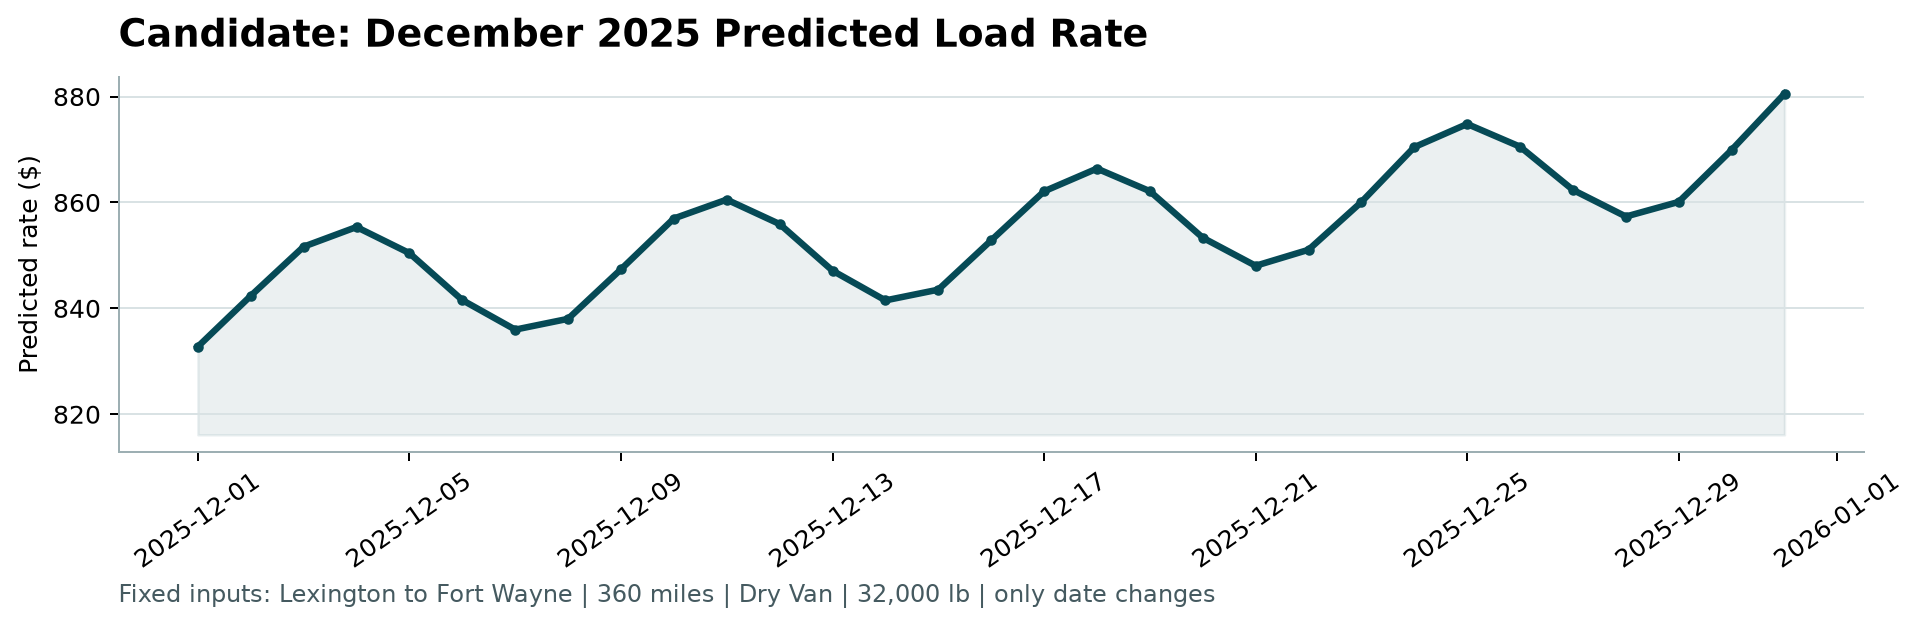
\includegraphics[width=\textwidth]{candidate_december.png}
\caption{The December chart produced by the provided \code{score.py}.}
\label{fig:december}
\end{figure}

The predicted rate rises from \$833 on 1 December to \$881 on 31 December
(Figure~\ref{fig:december}). Three things shape it: the weekly cycle of the market index,
which peaks on Thursdays; the dry van quarter-end premium, which builds through the month
to about 2.6\%; and the trend. Figure~\ref{fig:interval} adds the 90\% interval for a
single load. As a sanity check, the same lane and equipment posted between \$778 and \$865
in September and October, and between \$758 and \$934 over the year.

\begin{figure}[h]
\centering
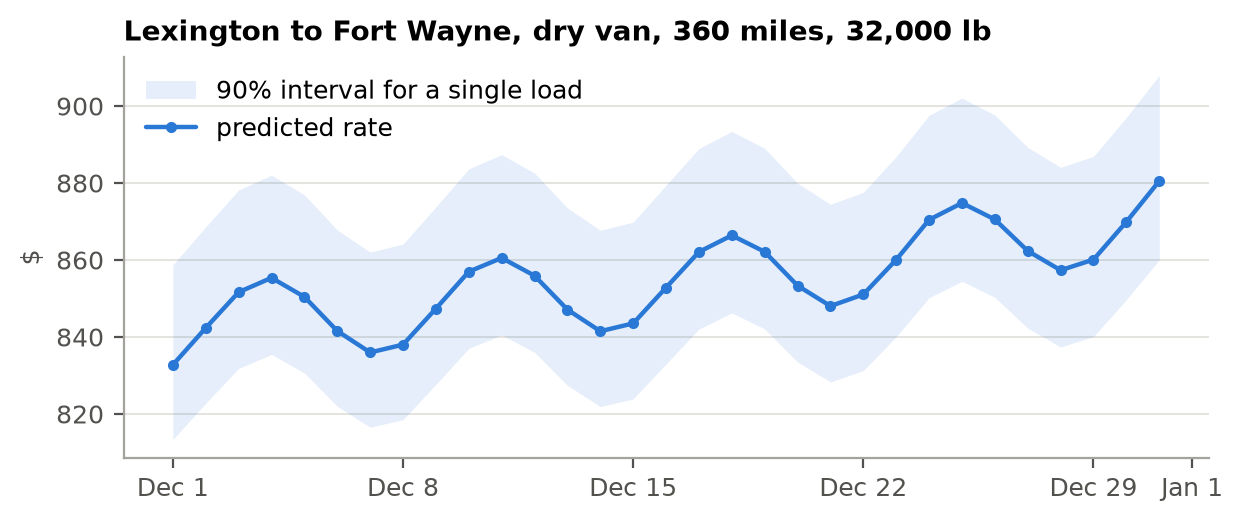
\includegraphics[width=0.9\textwidth]{december_interval.png}
\caption{The December series with a 90\% interval for one load on each day.}
\label{fig:interval}
\end{figure}

\section{Limitations}
\label{sec:limits}

\begin{itemize}
\item The trend is a straight line in log space carried two months past the data. Ten
months cannot show whether the drift changes at the end of the year. The daily residuals
are still autocorrelated (0.84 from one day to the next), so there is a slowly moving
level the features do not explain; on the September--October fold the model ended 1.3\%
low.
\item The fourth-quarter premium is assumed to match the first three quarters.
\item If the scoring metric were RMSE over all labels, corrupted ones included, raising
every prediction by about 1\% would score better. I did not, because the clean rate is
the number that is useful to price a load.
\item 12.2\% of validation loads are on lanes with no history and get no lane effect, and
the eight unseen cities are priced from their coordinates alone.
\end{itemize}

\section{Reproducing the results}
\label{sec:reproduce}

The code is at \url{\repo}. From a fresh clone:
\begin{verbatim}
python3 -m venv .venv
.venv/bin/pip install -r requirements.txt
.venv/bin/python -m pytest -q
.venv/bin/python -m ratecast backtest     # about 3 minutes
.venv/bin/python -m ratecast ablations    # Section 4.6, about 9 minutes
.venv/bin/python -m ratecast train
.venv/bin/python -m ratecast predict
.venv/bin/python score.py --predictions outputs/validation_predictions.csv \
    --december-predictions outputs/december_chart_inputs.csv \
    --output-dir outputs/scorer_results
\end{verbatim}
Results are deterministic. The tests cover the input checks, the calendar and market
features, the label screening on planted corruption, that every backtest fold trains only
on screened earlier loads, the trend extrapolation and lane shrinkage on synthetic data,
the template alignment and the interval calibration.

\end{document}
